% =====================================================================
%  Capitolo 1 — Elementi di calcolo degli intervalli
%  Apertura (p-05, p-06) trascritta integralmente.
%  Sezioni 1.1-1.3.3 (da p-07 in poi): DA TRASCRIVERE.
% =====================================================================
\chapter{Elementi di calcolo degli intervalli}

Esistono diversi modi attraverso i quali si può procedere all'investigazione
sulla natura e calcolo degli intervalli e tra questi, da quasi 3000 anni,
l'impiego del monocordo si è rivelato particolarmente efficace per esperimenti
e dimostrazioni di carattere scientifico e musicale. Il monocordo, come dice il
nome stesso, è uno strumento formato da una corda tesa tra due ponticelli su
una cassa di risonanza e da un ulteriore ponticello mobile che viene utilizzato
per dividere la corda in porzioni diverse a seconda dell'intervallo desiderato.

L'altezza di un suono generato su un monocordo dipende dal peso per unità di
lunghezza della corda (materiale e diametro), tensione e lunghezza. Queste
grandezze sono alla base delle quattro leggi fondamentali riguardanti la corda
vibrante in relazione all'altezza del suono emesso:

\begin{elenco}
  \item il numero di periodi per secondo è inversamente proporzionale alla
        lunghezza della corda;
  \item il numero di periodi per secondo è proporzionale alla radice quadrata
        della tensione alla quale la corda è soggetta;
  \item il numero di periodi per secondo varia inversamente allo spessore della
        corda;
  \item il numero di periodi per secondo è inversamente proporzionale alla
        radice quadrata della densità della corda.
\end{elenco}


Per il nostro scopo terremo conto soltanto della lunghezza della corda,
ritenendo costanti gli altri parametri. Ora, considerando la prima legge sulla
corda vibrante, avremo che se la corda è lunga un metro e oscilla con una
frequenza di 500 periodi al secondo, la stessa corda con il ponticello mobile
disposto alla sua metà ($1/2$) darà una frequenza pari a
$500 \times \frac{2}{1} = 1000$ periodi al secondo e, ancora, ridotta a $2/3$
della lunghezza totale, darà $500 \times \frac{3}{2} = 750$ periodi al secondo,
e così via. Nel calcolo della frequenza di un intervallo i termini del rapporto
che la definiscono verranno posti in modo tale da avere il valore più grande al
numeratore, mentre per determinare la lunghezza della corda vibrante il valore
più grande si troverà al denominatore. Poniamo di avere una corda lunga un metro
con una frequenza propria di 500~Hz: per sapere sia la frequenza relativa che il
punto della corda dove si dovrà disporre il ponticello mobile per trovare la sua
quinta ($3/2$) avremo:
\[
  500~\text{Hz} \times \tfrac{3}{2} = 750~\text{Hz}
  \qquad
  1~\text{m} \times \tfrac{2}{3} = 66{,}6~\text{cm}
\]

Un \emph{intervallo} tra due frequenze viene definito dal rapporto, o dal
quoziente, tra le due frequenze che lo formano. Per esempio, l'intervallo o la
distanza tra una frequenza di 500~Hz e una di 800~Hz è espresso dal rapporto
$8/5$ oppure dal suo quoziente $1{,}6$.

Nel calcolo teorico degli intervalli le altezze reali sono immaginarie: una nota
arbitraria, normalmente DO, viene scelta come punto di partenza e ad essa è
assegnato un valore di frequenza $1$. In pratica il calcolo degli intervalli
viene effettuato considerando essenzialmente tre intervalli elementari:
\[
  \text{ottava} = O \qquad
  \text{quinta} = Q \qquad
  \text{terza maggiore} = T
\]

Esperimenti iniziati da Pitagora da Samo già nel VI secolo a.C. fornirono le
seguenti regole:

\begin{elenco}
  \item la frequenza di un suono è $n$, quella dell'ottava è $2n$, della quinta
        $\frac{3}{2}n$ e della terza maggiore $\frac{5}{4}n$ (è da notare che
        questi intervalli sono i primi tre componenti con una propria identità
        della serie degli armonici: $2/1$ ottava, $3/1$ dodicesima-quinta,
        $5/1$ diciassettesima-terza maggiore);
  \item gli intervalli si \emph{addizionano} moltiplicando le loro rispettive
        frazioni. Quindi, per esempio, l'intervallo di dodicesima (quinta
        all'ottava superiore) è uguale a
        $Q + O = \frac{3}{2} \times \frac{2}{1} = \frac{3}{1}$;
        l'intervallo di settima maggiore è uguale a
        $Q + T = \frac{3}{2} \times \frac{5}{4} = \frac{15}{8}$;
  \item un intervallo si \emph{sottrae} moltiplicando la rispettiva frazione
        invertita. Per esempio, l'intervallo di quarta è uguale a
        $O - Q = \frac{2}{1} \times \frac{2}{3} = \frac{4}{3}$ e l'intervallo di
        terza minore è uguale a
        $Q - T = \frac{3}{2} \times \frac{4}{5} = \frac{6}{5}$.
\end{elenco}

Nel calcolo degli intervalli complessi si può procedere ad una semplificazione
che consiste nel non considerare l'intervallo nell'ambito del rapporto $2/1$,
trascurando cioè il fattore 2. Così facendo la quinta diviene semplicemente $3$
e la terza maggiore $5$. Naturalmente, con questo procedimento, le ottave
risultanti non sono corrette nel senso della posizione dell'intervallo
nell'ambito di una stessa ottava. Comunque questa piccola difficoltà può essere
facilmente risolta moltiplicando il risultato ottenuto per una potenza di 2
($2, 4, 8, \tfrac{1}{2}, \tfrac{1}{4}, \tfrac{1}{8}$ ecc.).

Grazie a questo calcolo si può far rientrare l'intervallo nell'ottava. Ad
esempio nel calcolo della settima maggiore si avrà:
\[
  Q + T = 3 \times 5 = 15 \times \tfrac{1}{8} = \tfrac{15}{8}
\]

Un intervallo è contenuto nell'ottava quando il valore del denominatore della
sua frazione è superiore alla metà del valore del numeratore e quindi il
risultato del quoziente è compreso tra 1 e 2.

Questo sistema di calcolo degli intervalli è particolarmente conveniente quando
si deve stabilire l'intervallo rispetto ad un rapporto dato. Per esempio, quale
intervallo è rappresentato da $9/8$? Trascurando tutte le potenze di 2 (quindi
8) troviamo che esso è formato da $3 \times 3 = 9$ cioè $Q + Q = $~RE, quindi
l'intervallo è di un tono. Oppure determinare l'intervallo corrispondente al
rapporto $25/18$:
\[
  \frac{25}{18} = \frac{5 \times 5}{3 \times 3 \times 2} = 2T - 2Q = \text{FA}\sharp
\]
e ancora, trovare l'intervallo corrispettivo al rapporto $45/32$:
\[
  45 = 3 \times 3 \times 5 = 2Q + T = \text{FA}\sharp
\]

Questo FA$\sharp$ non può essere uguale al primo e la ragione di tale
differenza, un \emph{comma sintonico}, è da ricercarsi nel fatto che il calcolo
di uno stesso intervallo può essere eseguito con diverse combinazioni di ottave,
quinte e terze maggiori.\footnote{I termini ottava, quinta e terza sono relativi
ai gradi della scala eptatonica dove, per esempio, il rapporto $2/1$ (ottava)
corrisponde appunto al suo ottavo grado. Chiaramente, per altre scale, come la
pentatonica o la dodecatonica, essi sono totalmente impropri. I Greci chiamavano
l'intervallo tra la corda intera e la sua metà \emph{diapason}, termine che
tradotto letteralmente significa \emph{attraverso tutto}, \emph{attraverso
l'intero}, ossia attraverso l'intero spazio tonale le cui relazioni interne si
ripetono sempre uguali.} Il sistema più semplice per calcolare la differenza o
\emph{comma sintonico} tra i due FA$\sharp$ consiste nel sottrarre i due membri
che li rappresentano:
\[
  (2Q+T) - (2T-2Q) = 2Q + T - 2T + 2Q = 4Q - T =
\]
\[
  = \tfrac{3}{2} \times \tfrac{3}{2} \times \tfrac{3}{2} \times \tfrac{3}{2}
    \times \tfrac{4}{5} = \tfrac{81}{20} \times \tfrac{1}{4}
    = \frac{81}{80}\footnote{La scrittura per esteso è stata adottata per
    maggiore chiarezza, ma naturalmente l'espressione può essere indicata come:
    $\left(\frac{3}{2}\right)^{4} \times \frac{4}{5} =
     \frac{81}{20} \times \frac{1}{4} = \frac{81}{80}$.}
\]

$81/80$ è il rapporto che rappresenta il \emph{comma sintonico}.

Ecco il calcolo del \emph{comma sintonico} tra il tono grande $9/8$, comune sia
al sistema pitagorico che a quello naturale, e il tono piccolo $10/9$ presente
solo in quello naturale:
\[
  \text{tono grande} = \frac{9}{8} = 2Q = \frac{3}{2} \times \frac{3}{2}
    = \frac{9}{4} \times \frac{1}{2} = \frac{9}{8}
\]
\[
  \text{tono piccolo} = \frac{10}{9} = O + T - 2Q = \frac{2}{1} \times
    \frac{5}{4} \times \frac{4}{9} = \frac{40}{36} = \frac{10}{9}
\]
\[
  \text{quindi} \quad (2Q) - (O - T - 2Q) = 2Q - O + T + 2Q = 4Q - O - T =
\]
\[
  = \tfrac{3}{2} \times \tfrac{3}{2} \times \tfrac{3}{2} \times \tfrac{3}{2}
    \times \tfrac{1}{2} \times \tfrac{4}{5} = \frac{324}{160} = \frac{81}{80}
\]
% [sic] Nell'originale il risultato intermedio 324/160 è ridotto a 81/80
% (la riduzione corretta sarebbe 81/40): refuso riprodotto fedelmente.

Il \emph{Comma} e lo \emph{Schisma} sono quei valori di scarto in altezza che si
vengono a determinare nel calcolo degli intervalli\footnote{Tale calcolo rimane
inalterato indipendentemente dalla natura del generatore, sia esso corda
vibrante o colonna d'aria in un tubo.} quando una stessa altezza, come abbiamo
già avuto modo di vedere, viene ottenuta attraverso la differente combinazione
di ottave, quinte e terze maggiori.\footnote{Tutti gli intervalli, ad eccezione
dell'ottava che è comune a tutti i sistemi di intonazione, sono da considerarsi
come riferiti al sistema naturale e non a quello del temperamento equabile.}

Il \emph{Comma ditonico} o \emph{pitagorico} si verifica nella differenza tra 12
quinte e 7 ottave $(12Q - 7O)$:
\[
  \left(\frac{3}{2}\right)^{12} \times \left(\frac{1}{2}\right)^{7}
  = \frac{3^{12}}{2^{19}} = \frac{531441}{524288}
  = 23{,}5~\text{cents}\footnote{Per il calcolo dei cents vedi
  \emph{Intervalli logaritmici}.}
\]

Il \emph{Comma sintonico} o \emph{Didimico} si verifica nella differenza tra 4
quinte e la somma di 2 ottave più una terza maggiore $(4Q - 2O - 1T)$:
\[
  \left(\frac{3}{2}\right)^{4} \times \frac{4}{5} \times
  \left(\frac{1}{2}\right)^{2} = \frac{3^{4}}{2^{4} \times 5}
  = \frac{81}{80} = 21{,}5~\text{cents}
\]

Lo \emph{Schisma} si verifica nella differenza tra 8 quinte più una terza
maggiore e 5 ottave $(8Q + 1T - 5O)$:
\[
  \left(\frac{3}{2}\right)^{8} \times \frac{5}{4} \times
  \left(\frac{1}{2}\right)^{5} = \frac{3^{8} \times 5}{2^{15}}
  = \frac{32805}{32768} = 2~\text{cents}
\]

Il \emph{Diaschisma} si verifica nella differenza tra 3 ottave e la somma di 4
quinte più 2 terze maggiori $(3O - 4Q - 2T)$:
\[
  \left(\frac{2}{1}\right)^{3} \times \left(\frac{2}{3}\right)^{4} \times
  \left(\frac{4}{5}\right)^{2} = \frac{2^{11}}{3^{4} \times 5^{2}}
  = \frac{2048}{2025} = 19{,}5~\text{cents}
\]

Il \emph{comma ditonico} è anche la differenza tra i due semitoni della scala
diatonica pitagorica e il \emph{comma sintonico}, come visto precedentemente,
tra i due toni interi della scala naturale.

Lo \emph{schisma} è la differenza tra il \emph{comma ditonico} e quello
\emph{sintonico}, nonché tra il \emph{comma sintonico} e il \emph{diaschisma}:
\[
  \frac{3^{12}}{2^{19}} \times \frac{5 \times 2^{4}}{3^{4}}
  = \frac{3^{8} \times 5}{2^{15}}
\]
\[
  \frac{3^{4}}{2^{4} \times 5} \times \frac{3^{4} \times 5^{2}}{2^{11}}
  = \frac{3^{8} \times 5}{2^{15}}
\]

% =====================================================================
\section{Intervalli complementari}

Due intervalli si dicono complementari quando, moltiplicando le rispettive
frazioni, il risultato che si ottiene è $2/1$. Ad esempio, moltiplicando
$3/2 \times 4/3$ si otterrà:
\[
  \frac{3}{2} \times \frac{4}{3} = \frac{4}{2} = \frac{2}{1}
\]

Dato un intervallo, il complementare si ricava semplicemente invertendo i suoi
due termini, facendo però attenzione che la nuova frazione sia stata prima
semplificata (ridotta ai minimi termini) e che essa sia contenuta nell'ambito
dell'ottava. Ne risulta che il complementare di $81/80$ sarà $80/81$ che
riportato nell'ottava darà $160/81$. Pertanto:
\[
  \frac{81}{80} \times \frac{160}{81} = \frac{160}{80} = \frac{2}{1}
\]

Trovare il complementare di $800/729$: invertendo i termini della frazione
avremo $729/800$. Riportandola nell'ottava avremo $1458/800$ che, ridotta ai
minimi termini, risulterà $729/400$, quindi:
\[
  \frac{800}{729} \times \frac{729}{400} = \frac{800}{400} = \frac{2}{1}
\]

Naturalmente, l'intervallo complementare si può ottenere anche moltiplicando la
frazione che lo esprime per $1/2$ e invertendo poi il risultato ottenuto:
\[
  \frac{15}{8} \times \frac{1}{2} = \frac{15}{16} \quad\text{da cui}\quad
  \frac{16}{15}
\]

% =====================================================================
\section{Intervalli logaritmici}

L'impiego dei logaritmi può semplificare molto il calcolo degli intervalli.
Secondo l'equazione fondamentale dei logaritmi:
\[
  \log(A \times B) = \log A + \log B
\]
ne consegue che il logaritmo di un prodotto è uguale alla somma dei logaritmi
dei fattori. Vale a dire $\log 15 = \log 3 + \log 5$. Se perciò due intervalli
$i_1$ e $i_2$ sono rappresentati non dai loro rapporti di frequenza $f_1$ e
$f_2$ ma dai logaritmi dei simboli $\log f_1$ e $\log f_2$, il calcolo degli
intervalli viene effettuato con:
\[
  \log(f_1 \times f_2) = \log f_1 + \log f_2
\]

Si ottiene così che, se vengono usati gli intervalli logaritmici, l'addizione e
la sottrazione degli intervalli viene fatta in realtà addizionando e sottraendo
i simboli anziché moltiplicandoli o dividendoli. Il vantaggio principale
nell'impiego delle frequenze logaritmiche consiste nel fatto che uguali
intervalli musicali sono rappresentati da uguali distanze su una scala
geometrica.

\begin{figure}[htbp]
  \centering
  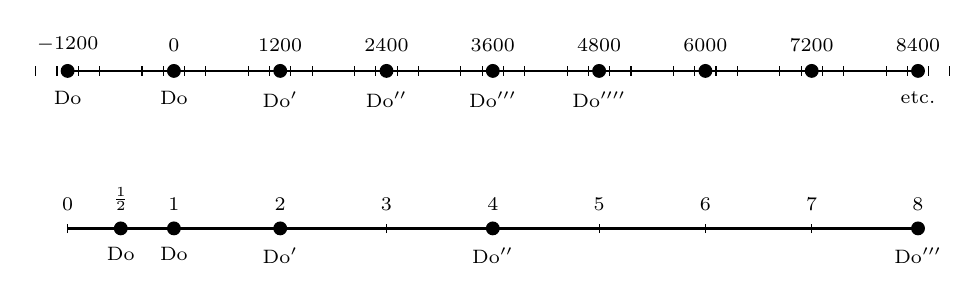
\begin{tikzpicture}[x=1.35cm,y=1cm]
    % --- (a) scala logaritmica (cents): le ottave sono equidistanti ---
    \draw[thick] (0,2) -- (8,2);
    \foreach \i in {0,...,8}{
      \foreach \k in {1,...,4}{\draw (\i-0.5+\k*0.2,1.94) -- (\i-0.5+\k*0.2,2.06);}
    }
    \foreach \i/\n/\d in {%
        0/$-1200$/Do, 1/$0$/Do, 2/$1200$/Do$'$, 3/$2400$/Do$''$,
        4/$3600$/Do$'''$, 5/$4800$/Do$''''$, 6/$6000$/{}, 7/$7200$/{},
        8/$8400$/etc.}{
      \filldraw (\i,2) circle (2.3pt);
      \node[above,font=\scriptsize] at (\i,2.12) {\n};
      \node[below,font=\scriptsize] at (\i,1.86) {\d};
    }
    % --- (b) scala lineare (frequenza): le ottave si allontanano ---
    \draw[thick] (0,0) -- (8,0);
    \foreach \i in {0,...,8}{\draw (\i,-0.06) -- (\i,0.06);}
    \draw (0.5,-0.06) -- (0.5,0.06);
    \foreach \x/\n in {0/$0$,0.5/$\frac12$,1/$1$,2/$2$,3/$3$,4/$4$,5/$5$,6/$6$,7/$7$,8/$8$}
      {\node[above,font=\scriptsize] at (\x,0.10) {\n};}
    \foreach \x/\d in {0.5/Do,1/Do,2/Do$'$,4/Do$''$,8/Do$'''$}{
      \filldraw (\x,0) circle (2.3pt);
      \node[below,font=\scriptsize] at (\x,-0.12) {\d};
    }
  \end{tikzpicture}
\end{figure}

Dall'esempio si vede come nella usuale scala logaritmica dei cents le varie
ottave sono indicate da cifre equidistanti, come $0$, $1200$, $2400$, $3600$
cents, mentre al contrario, nella scala lineare delle frequenze, le ottave sono
indicate dalle cifre $1$, $2$, $4$, $8$ ecc. Le frequenze logaritmiche sono
particolarmente importanti, se non indispensabili, in tutti i calcoli inerenti
intervalli temperati o microintervalli. Ad esempio, il temperamento equabile
consiste nella divisione dell'ottava in 12 intervalli (semitoni) equidistanti.
Poiché l'ottava ha la frequenza 2, abbiamo l'equazione
$\sqrt[12]{2}$,\footnote{Il calcolo della radice $n$-esima di un numero
$\sqrt[n]{a}$ si effettua con $a^{1/n}$. Per esempio, nel caso di
$\sqrt[12]{2}$ si procederà nel dividere 1 per l'indice del radicale:
$1/12 = 0{,}083333\ldots$, quindi si eleverà il radicando 2 per il risultato
ottenuto: $2^{0{,}083333\ldots} = 1{,}059463094$.} quindi $1{,}0594630943$. La
successiva potenza di questa cifra darà la frequenza dell'intervallo seguente
della scala temperata: $\text{RE} = 1{,}05946^{2} = 1{,}12246$,
$\text{RE}\sharp = 1{,}05946^{3} = 1{,}18919$ ecc.

Usando invece i logaritmi, gli intervalli della scala temperata possono essere
calcolati facilmente essendo essi tutti multipli del $\log$ dell'intervallo più
piccolo: $\log 1{,}0594630943 = 0{,}025085833$, quindi $\text{DO} = 0$,
$\text{DO}\sharp = 0{,}025085833$, $\text{RE} = 0{,}050171666$,
$\text{RE}\sharp = 0{,}075257499$ e così via fino all'ottava
$\text{DO'} = 0{,}301029957$.

L'unico inconveniente in questo sistema di calcolo è rappresentato dal fatto di
dover impiegare numeri così ingombranti. Tuttavia questa difficoltà può essere
facilmente evitata moltiplicando la scala per un determinato fattore. In questo
modo allargato si ottengono varie scale logaritmiche. La più diffusa è quella
studiata da Ellis [Alexander J. Ellis, 1814--1890] nella quale il fattore
allargato è dato da $1200/\!\log 2 = 3986{,}313714$, cosicché l'ottava viene
divisa esattamente in 1200 parti. L'unità, in questo sistema di misurazione, è
il \emph{cent}. Quindi, se l'ottava divisa in 12 semitoni equidistanti è uguale
a $1200$ cents, ogni semitono temperato avrà il valore di $100$ cents.

Un altro sistema logaritmico piuttosto comune è quello di Savart [Felix Savart,
1791--1841]. Anche con questa scala è possibile calcolare gli intervalli
logaritmici contenuti nell'ambito del rapporto $2/1$, ossia tra $0$ e $0{,}3010$.
In questo metodo il fattore allargato è uguale a $1000$, quindi tutte le cifre
vengono moltiplicate per $1000$ ottenendo così che l'ottava, anziché essere
$0{,}3010$, è uguale a $301$ savarts. Entrambi i sistemi sono molto efficaci per
calcolare qualsiasi tipo di intervallo musicale. Difatti, se consideriamo che il
semitono temperato nel sistema di Ellis corrisponde a $100$ cents, si possono
prevedere misurazioni agevolmente fino ad $1/100$ di semitono.

Leonardo Eulero [1707--1783] già utilizzava i logaritmi per la definizione della
grandezza degli intervalli, presentati sotto forma di rapporti matematici tra le
loro rispettive frequenze $(i/i')$. Considerando l'ottava intervallo musicale
fondamentale, Eulero inizialmente utilizzò logaritmi decimali, sostituendoli poi
con quelli a base 2, attribuendo così all'ottava la cifra $1$. Nel 1834 F. W.
Opitz combinò il concetto di Eulero dell'ottava come intervallo di base con
l'idea di Savart dell'estensione fino a $1000$, suggerendo di calcolare i
rapporti di frequenza secondo la formula:
\[
  x = 1000 \log_2 i/i'
\]

Questa formula venne adottata anche da Arthur Joachim von Oettingen
[1836--1920], che introdusse il termine \emph{milli-ottava}. Un passo importante
verso un ulteriore chiarimento sulla misurazione della trasformazione
logaritmica venne compiuto da Baron Riche de Prony, il quale utilizzò come unità
operativa il mezzo tono temperato:
\[
  x = \frac{12}{\log 2} \times \log i/i'
\]
Questa formula venne elaborata poi da Gottfried Heinrich Bellermann
[1832--1908], il quale propose $100$ come unità di misura per il mezzo tono
temperato al posto di $1$\footnote{Il calcolo della radice n-esima di un numero 
$\sqrt[n]{a}$ si effettua con: $\frac{1}{a^n}$. Per esempio, nel caso di $\sqrt[12]{2}$
si procederà nel dividere 1 per l'indice del radicale: $1/12 = 0{,}08\overline{3 }$ \ldots
quindi si eleverà il radicando 2 per il risultato ottenuto: $2^{0{,}08\overline{3}} = 1{,}059463094\ldots$}.

% =====================================================================
\section{Conversione rapporto/cents/rapporto}

Nello studio dei sistemi di intonazione e nel calcolo degli intervalli è molto
frequente e necessaria la conversione di intervalli da una scala di misurazione
ad un'altra. Tuttavia, prima di passare ad analizzare i più frequenti tipi di
conversioni, potrà tornare utile vedere brevemente quali sono le proprietà
generali dei rapporti, dato che un intervallo è sempre rappresentato da un
rapporto.

I rapporti possiedono quattro proprietà:
\begin{elenco}
  \item un rapporto è costituito da due numeri interi positivi;
  \item ogni rapporto appartiene ad una famiglia di rapporti equivalenti;
  \item dato un qualsiasi rapporto, si può ottenere un rapporto ad esso
        equivalente dividendo ciascun termine per un fattore comune;
  \item dato un qualsiasi rapporto, si può ottenere un rapporto ad esso
        equivalente moltiplicando ciascun termine per un fattore comune.
\end{elenco}

Le proprietà 3) e 4) sono le stesse di quelle riguardanti la riduzione delle
frazioni ai minimi o ai massimi termini. Pertanto un rapporto è essenzialmente
una frazione e possiamo quindi usare la notazione frazionaria per
rappresentarlo: invece di scrivere $a:b$ possiamo scrivere la frazione $a/b$.

Una \emph{proporzione} è una uguaglianza di rapporti. Se $a/b$ è equivalente a
$c/d$, tale uguaglianza viene espressa in $a:b = c:d$ oppure $a/b = c/d$. In una
proporzione i numeri $a$ e $d$ vengono chiamati \emph{estremi} e i numeri $b$ e
$c$ \emph{medi}.

La proprietà fondamentale di una proporzione è che \emph{il prodotto dei medi è
uguale al prodotto degli estremi}. Se uno dei quattro termini della proporzione
è incognito, tale proprietà può essere utilizzata per identificarlo. Ad
esempio, nella proporzione $2:4 = 5:x$ che, scritta sotto la forma di frazione,
sarà:
\[
  \frac{2}{4} = \frac{5}{x}
\]
si potrà applicare la proprietà dell'equivalenza delle frazioni per trovare che
$2x = 20$, quindi dividendo entrambi i membri dell'equazione per 2, oppure
moltiplicandoli per $1/2$, troveremo che $x = 10$.

\subsection{Conversione da rapporto in cents}

Per la conversione di un rapporto in cents si dovrà procedere prima di tutto
alla risoluzione della frazione che lo esprime in decimale:
\[
  \frac{3}{2} = 3:2 = 1{,}5
\]
quindi si dovrà trovare il logaritmo del quoziente così ottenuto:
\[
  \log 1{,}5 = 0{,}1761
\]
ed infine il logaritmo del rapporto va moltiplicato per il fattore di
conversione di Ellis:
\[
  0{,}1761 \times (\frac{1200}{\log 2} = 0{,}1761 \times 3986{,}313714\ldots)
  = 702~\text{cents}\footnote{Tutti i valori in cents sono approssimati.}
\]
La stessa conversione in \textit{savarts} risulterà come:
\[
  3:2 = 1{,}5 \qquad \log 1{,}5 = 0{,}1761 \times 1000 = 176~\text{savarts}
\]

\subsection{Conversione da cents a numero decimale}

Questa operazione, che in sostanza è il contrario della precedente, si risolve
dividendo il numero dei cents per il fattore di conversione e dal risultato
ottenuto va ricavato l'antilogaritmo.
\[
  \text{Es.}\quad \frac{702~\text{cents}}{3986{,}313714} = 0{,}1761
\]
L'antilogaritmo di $0{,}1761$ è $1{,}5$.

\subsection{Conversione da un numero decimale in rapporto}

Sapendo che un rapporto viene comunemente espresso sottoforma di frazione, un
numero decimale finito o periodico si può ridurre ad una frazione che si chiama
\emph{frazione generatrice} del numero decimale.

Un numero decimale finito si riduce alla sua frazione generatrice scrivendo una
frazione che ha per numeratore il numero senza la virgola e come denominatore
l'unità seguita da tanti zeri quante sono le cifre decimali del numero.
\[
  \text{Es.}\quad 1{,}5 = \frac{15}{10} = \frac{3}{2}
  \qquad\text{oppure}\qquad 1{,}25 = \frac{125}{100} = \frac{5}{4}
\]

La generatrice di un numero periodico è una frazione che ha per numeratore la
differenza tra tutto il numero, senza la virgola, ed il numero formato dalle
cifre che precedono il periodo (parte intera e antiperiodo) e per denominatore
un numero formato da tanti 9 quante sono le cifre del periodo, seguito da tanti
zeri quante sono le cifre dell'antiperiodo (se c'è).
\begin{gather*}
  \text{Es.}\quad 1{,}\overline{3} = \frac{133-1}{99} = \frac{132}{99}
  = \frac{4}{3} \\[2pt]
  \text{oppure}\quad
  1{,}4\overline{2} = \frac{142-14}{90} = \frac{128}{90} = \frac{64}{45}
\end{gather*}

